\documentclass[UTF8]{ctexrep}

\usepackage{fancyhdr}
\usepackage[letterpaper, left=1in, right=1in, top=1in, bottom=1in]{geometry}
\usepackage{sectsty}
\usepackage{graphicx}
\usepackage{subfig}
\usepackage[section]{placeins}
\usepackage{hyperref}
\usepackage{amsmath}
\usepackage{listings}
\usepackage{color}
\usepackage{lstautogobble}

\definecolor{dkgreen}{rgb}{0,0.6,0}
\definecolor{gray}{rgb}{0.5,0.5,0.5}
\definecolor{mauve}{rgb}{0.58,0,0.82}

\lstset{frame=tb,
    language            = C,
    aboveskip           = 3mm,
    belowskip           = 5mm,
    showstringspaces    = false,
    columns             = flexible,
    basicstyle          = {\small\ttfamily},
    numbers             = none,
    numberstyle         = \tiny\color{gray},
    keywordstyle        = \color{blue},
    commentstyle        = \color{dkgreen},
    stringstyle         = \color{mauve},
    breaklines          = true,
    breakatwhitespace   = true,
    tabsize             = 3,
    numbers             = left,
    numberblanklines    = true,
    firstnumber         = 1,
    numberstyle         = \scriptsize\color{black},
    numbersep           = 12pt,
    escapeinside        = ||,
    mathescape          = true,
    autogobble          = true
}

\usepackage{xcolor}

\definecolor{codegreen}{rgb}{0,0.6,0}
\definecolor{codegray}{rgb}{0.5,0.5,0.5}
\definecolor{codepurple}{rgb}{0.58,0,0.82}
\definecolor{backcolour}{rgb}{0.95,0.95,0.92}

\lstdefinestyle{mystyle}{
    backgroundcolor=\color{backcolour},
    commentstyle=\color{codegreen},
    keywordstyle=\color{magenta},
    numberstyle=\tiny\color{codegray},
    stringstyle=\color{codepurple},
    basicstyle=\ttfamily\footnotesize,
    breaklines=true,
    captionpos=b,
    keepspaces=true,
    showspaces=false,
    showstringspaces=false,
    showtabs=false,
    tabsize=4
}

\lstset{style=mystyle}
\let\origthelstnumber\thelstnumber
\makeatletter
\newcommand*\Suppressnumber{%
  \lst@AddToHook{OnNewLine}{%
    \let\thelstnumber\relax%
     \advance\c@lstnumber-\@ne\relax%
    }%
}

\newcommand*\Reactivatenumber[1]{%
  \setcounter{lstnumber}{\numexpr#1-1\relax}
  \lst@AddToHook{OnNewLine}{%
   \let\thelstnumber\origthelstnumber%
   \refstepcounter{lstnumber}
  }%
}


\makeatother
\hypersetup{
    colorlinks=true,
    linkcolor=blue,
    filecolor=magenta,
    urlcolor=cyan,
}
\allsectionsfont{\mdseries\scshape}

\renewcommand{\thesection}{\arabic{section}}

\newcommand{\horrule}[1]{\rule{\linewidth}{#1}}
\title{
    \horrule{0.5pt} \\[0.4cm]
    \huge Project 3 \\
    \horrule{2pt}
}
\author{
    陈思贝 (718030290013)
}
\date{
    % TODO: Date
}
\setcounter{section}{-1}

\begin{document}
    \maketitle

    \section{实验配置}

    \begin{itemize}
        \item Linux Kernel: 4.15.0
        \item OS: Ubuntu 18.04.5 LTS
    \end{itemize}
    \vspace{.3cm}

    \section{实验过程}
    
    \texttt{mtest}模块加载后即会生成一个\texttt{/proc/mtest}文件。利用实验一中掌握的对\texttt{/proc}文件的操作,实现模块对于不同输入的操作与反馈。\\

    \subsection{listvma}

    该模块会列出当前进程的所有虚拟内存的地址。其中\texttt{vm\_area\_struct}的定义在\texttt{linux/mm\_types.h}文件中。\texttt{vm\_start}和\texttt{vm\_end}分别指向了vma的起始地址。这是一个双向链表,\texttt{vm\_next}指向了下一个vma,只需用循环就可遍历所有虚拟内存的地址并输出。

    \begin{lstlisting}[firstnumber=280]
    struct vm_area_struct {
        /* The first cache line has the info for VMA tree walking. */

        unsigned long vm_start;		/* Our start address within vm_mm. */
        unsigned long vm_end;		/* The first byte after our end address
                                    within vm_mm. */

        /* linked list of VM areas per task, sorted by address */
        struct vm_area_struct *vm_next, *vm_prev; |\Suppressnumber|
        $\dots$|\Reactivatenumber{303}|
        unsigned long vm_flags;		/* Flags, see mm.h. */|\Suppressnumber|
        $\dots$|\Reactivatenumber{509}|
    } __randomize_layout;
    \end{lstlisting}

    \texttt{vm\_flags}可以判断vma的读写执行权限,在\texttt{linux/mm.h}中有定义宏,只需将\texttt{vm\_flags}和相应的宏进行二元操作,就可以计算出相对应的权限。实际运行结果见图\ref{fig:listvma}。

    \begin{lstlisting}[firstnumber=172]
    #define VM_READ		0x00000001	/* currently active flags */
    #define VM_WRITE	0x00000002
    #define VM_EXEC		0x00000004
    \end{lstlisting}

    \subsection{findpage}

    该模块输入一个虚拟内存地址,会输出该虚拟地址在操作系统中所对应的物理内存的地址。本次实验所用的Linux系统仍然采用了四级分页的机制,其中分页的定义位于\texttt{arch/arm64/include/asm/pgtable-types.h}和\texttt{arch/arm64/include/asm/pgtable.h}中。分别为\texttt{pte}、\texttt{pmd}、\texttt{pud}和\texttt{pgd}四层分页。

    \begin{lstlisting}[firstnumber=25]
        typedef u64 pteval_t;
        typedef u64 pmdval_t;
        typedef u64 pudval_t;
        typedef u64 pgdval_t;
    \end{lstlisting}

    其中还定义了大量的分页位移宏,通过这些宏,可以通过多次映射,计算出虚拟内存地址所对应的物理内存地址。然后通过返回的页物理地址和虚拟地址的偏移量相结合,计算出最终的物理内存地址。测试结果见图\ref{fig:findpage}。

    \begin{lstlisting}[firstnumber=425]
        #define pte_offset_phys(dir,addr)	(pmd_page_paddr(READ_ONCE(*(dir))) + pte_index(addr) * sizeof(pte_t))
        #define pte_offset_kernel(dir,addr)	((pte_t *)__va(pte_offset_phys((dir), (addr))))

        #define pte_offset_map(dir,addr)	pte_offset_kernel((dir), (addr))
        #define pte_offset_map_nested(dir,addr)	pte_offset_kernel((dir), (addr))|\Suppressnumber|
        $\dots$|\Reactivatenumber{476}|
        #define pmd_offset_phys(dir, addr)	(pud_page_paddr(*(dir)) + pmd_index(addr) * sizeof(pmd_t))
        #define pmd_offset(dir, addr)		((pmd_t *)__va(pmd_offset_phys((dir), (addr))))|\Suppressnumber|
        $\dots$|\Reactivatenumber{528}|
        #define pud_offset_phys(dir, addr)	(pgd_page_paddr(*(dir)) + pud_index(addr) * sizeof(pud_t))
        #define pud_offset(dir, addr)		((pud_t *)__va(pud_offset_phys((dir), (addr))))
        #define pgd_offset_raw(pgd, addr)	((pgd) + pgd_index(addr))|\Suppressnumber|
        $\dots$|\Reactivatenumber{558}|
        #define pgd_offset(mm, addr)	(pgd_offset_raw((mm)->pgd, (addr)))

        /* to find an entry in a kernel page-table-directory */
        #define pgd_offset_k(addr)	pgd_offset(&init_mm, addr)

    \end{lstlisting}

    \subsection{writeval}

    该模块接受两个值,分别为1个虚拟内存地址和1个数值,并将数值写入虚拟内存的地址。通过\texttt{find\_vma}先找到vma的地址,并检验合格性,再检测是否为可写入的页。

    再通过上一个模块的\texttt{find\_page}计算出虚拟地址对应的物理地址,直接将数值写入该物理地址即可。测试结果见\ref{fig:writeval}。\\

    \section{实验效果截图}

    \begin{figure}[h!]
        \centering
        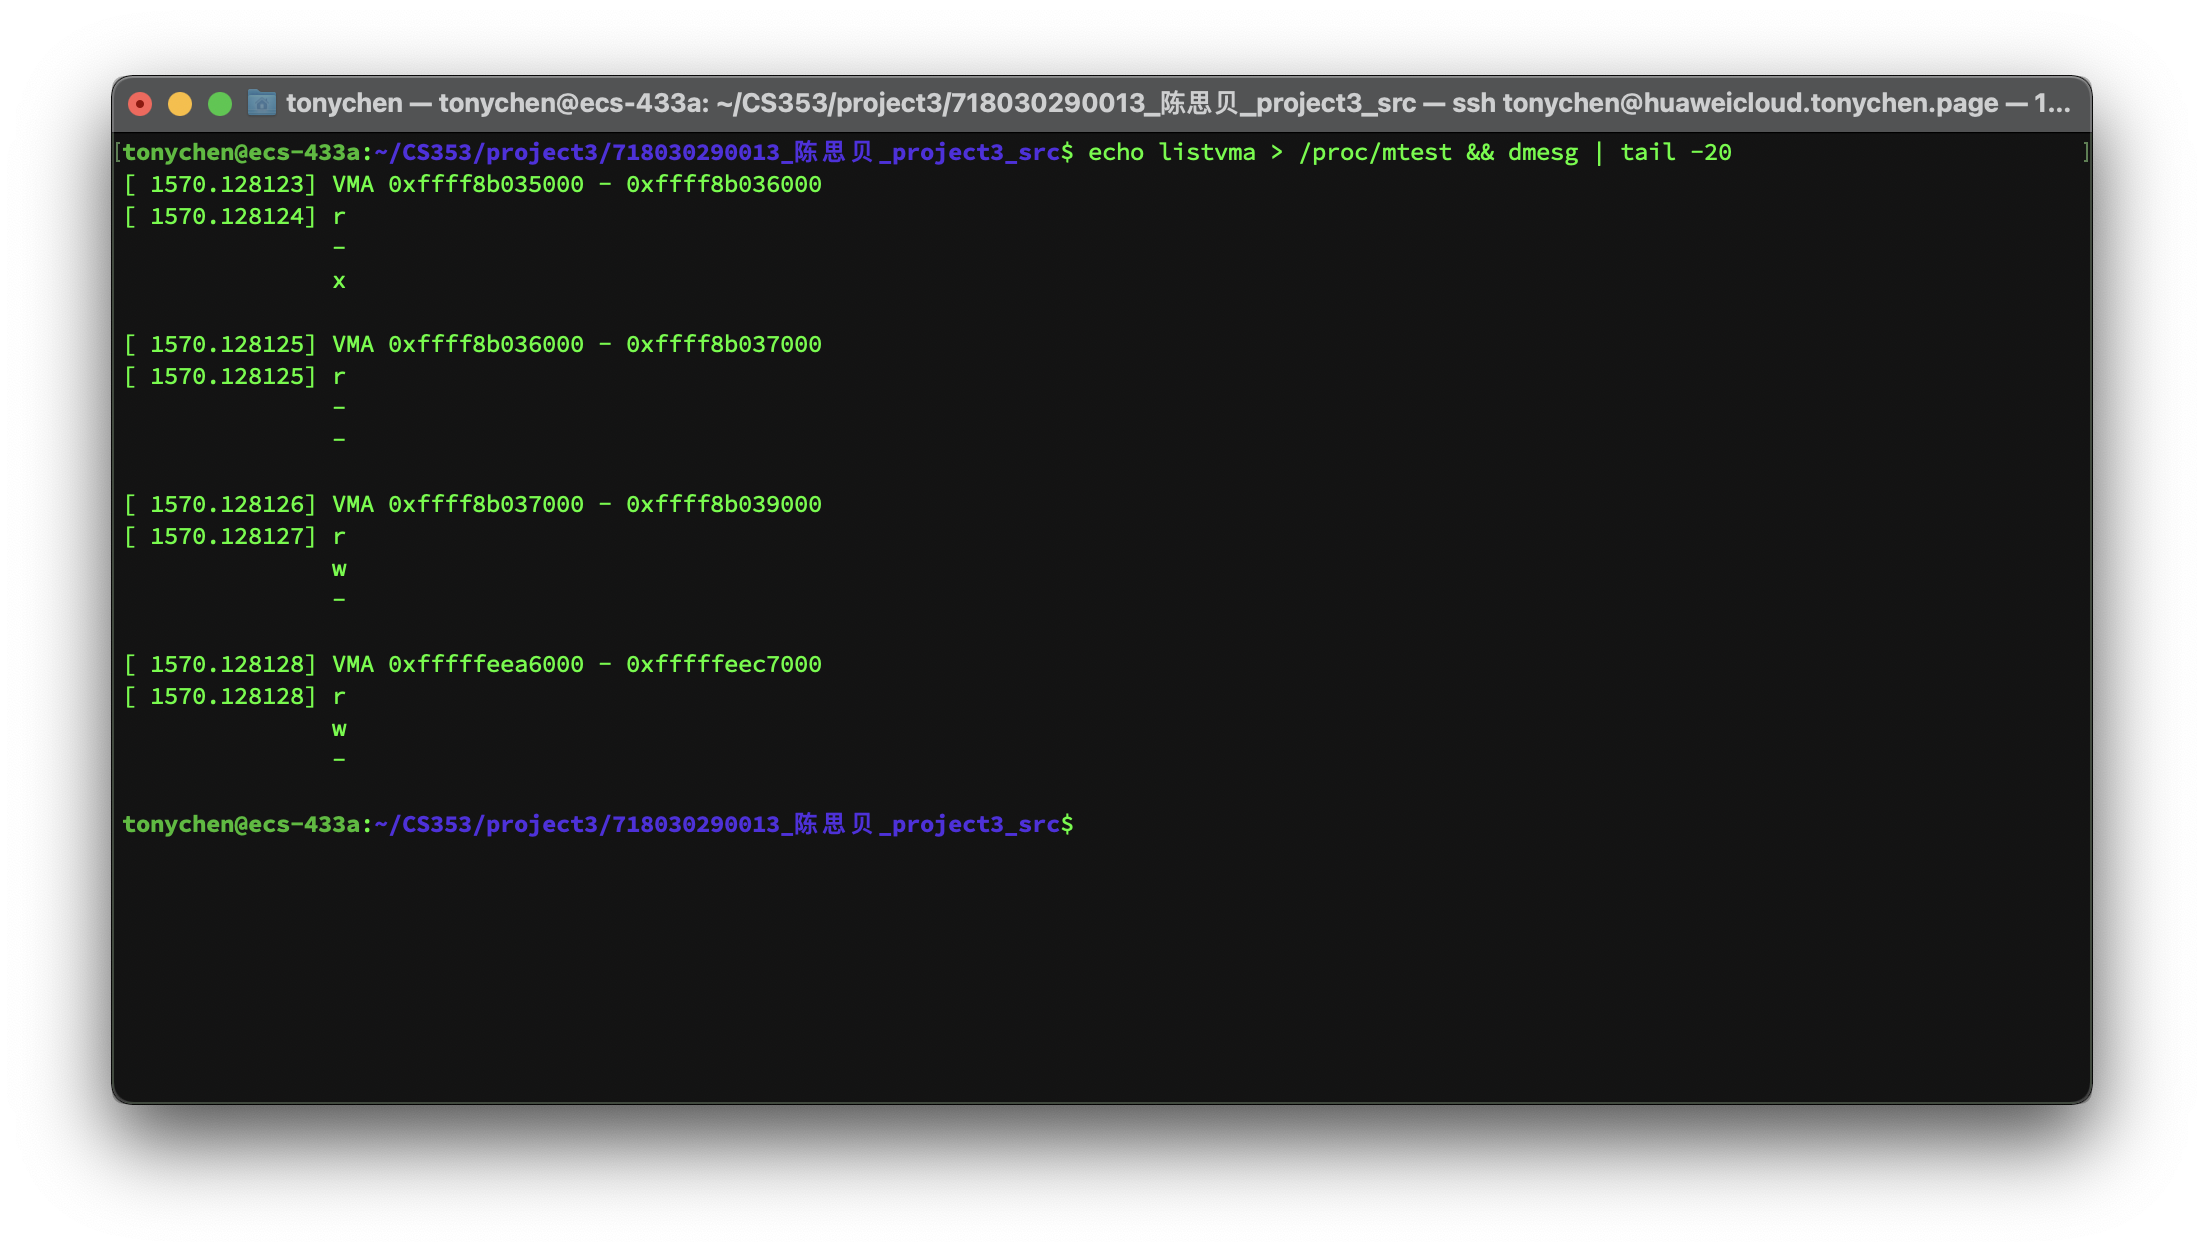
\includegraphics[width=15cm,keepaspectratio]{images/listvma.png}
        \caption{\texttt{listvma}部分运行结果}
        \label{fig:listvma}
    \end{figure}

    \begin{figure}[h!]
        \centering
        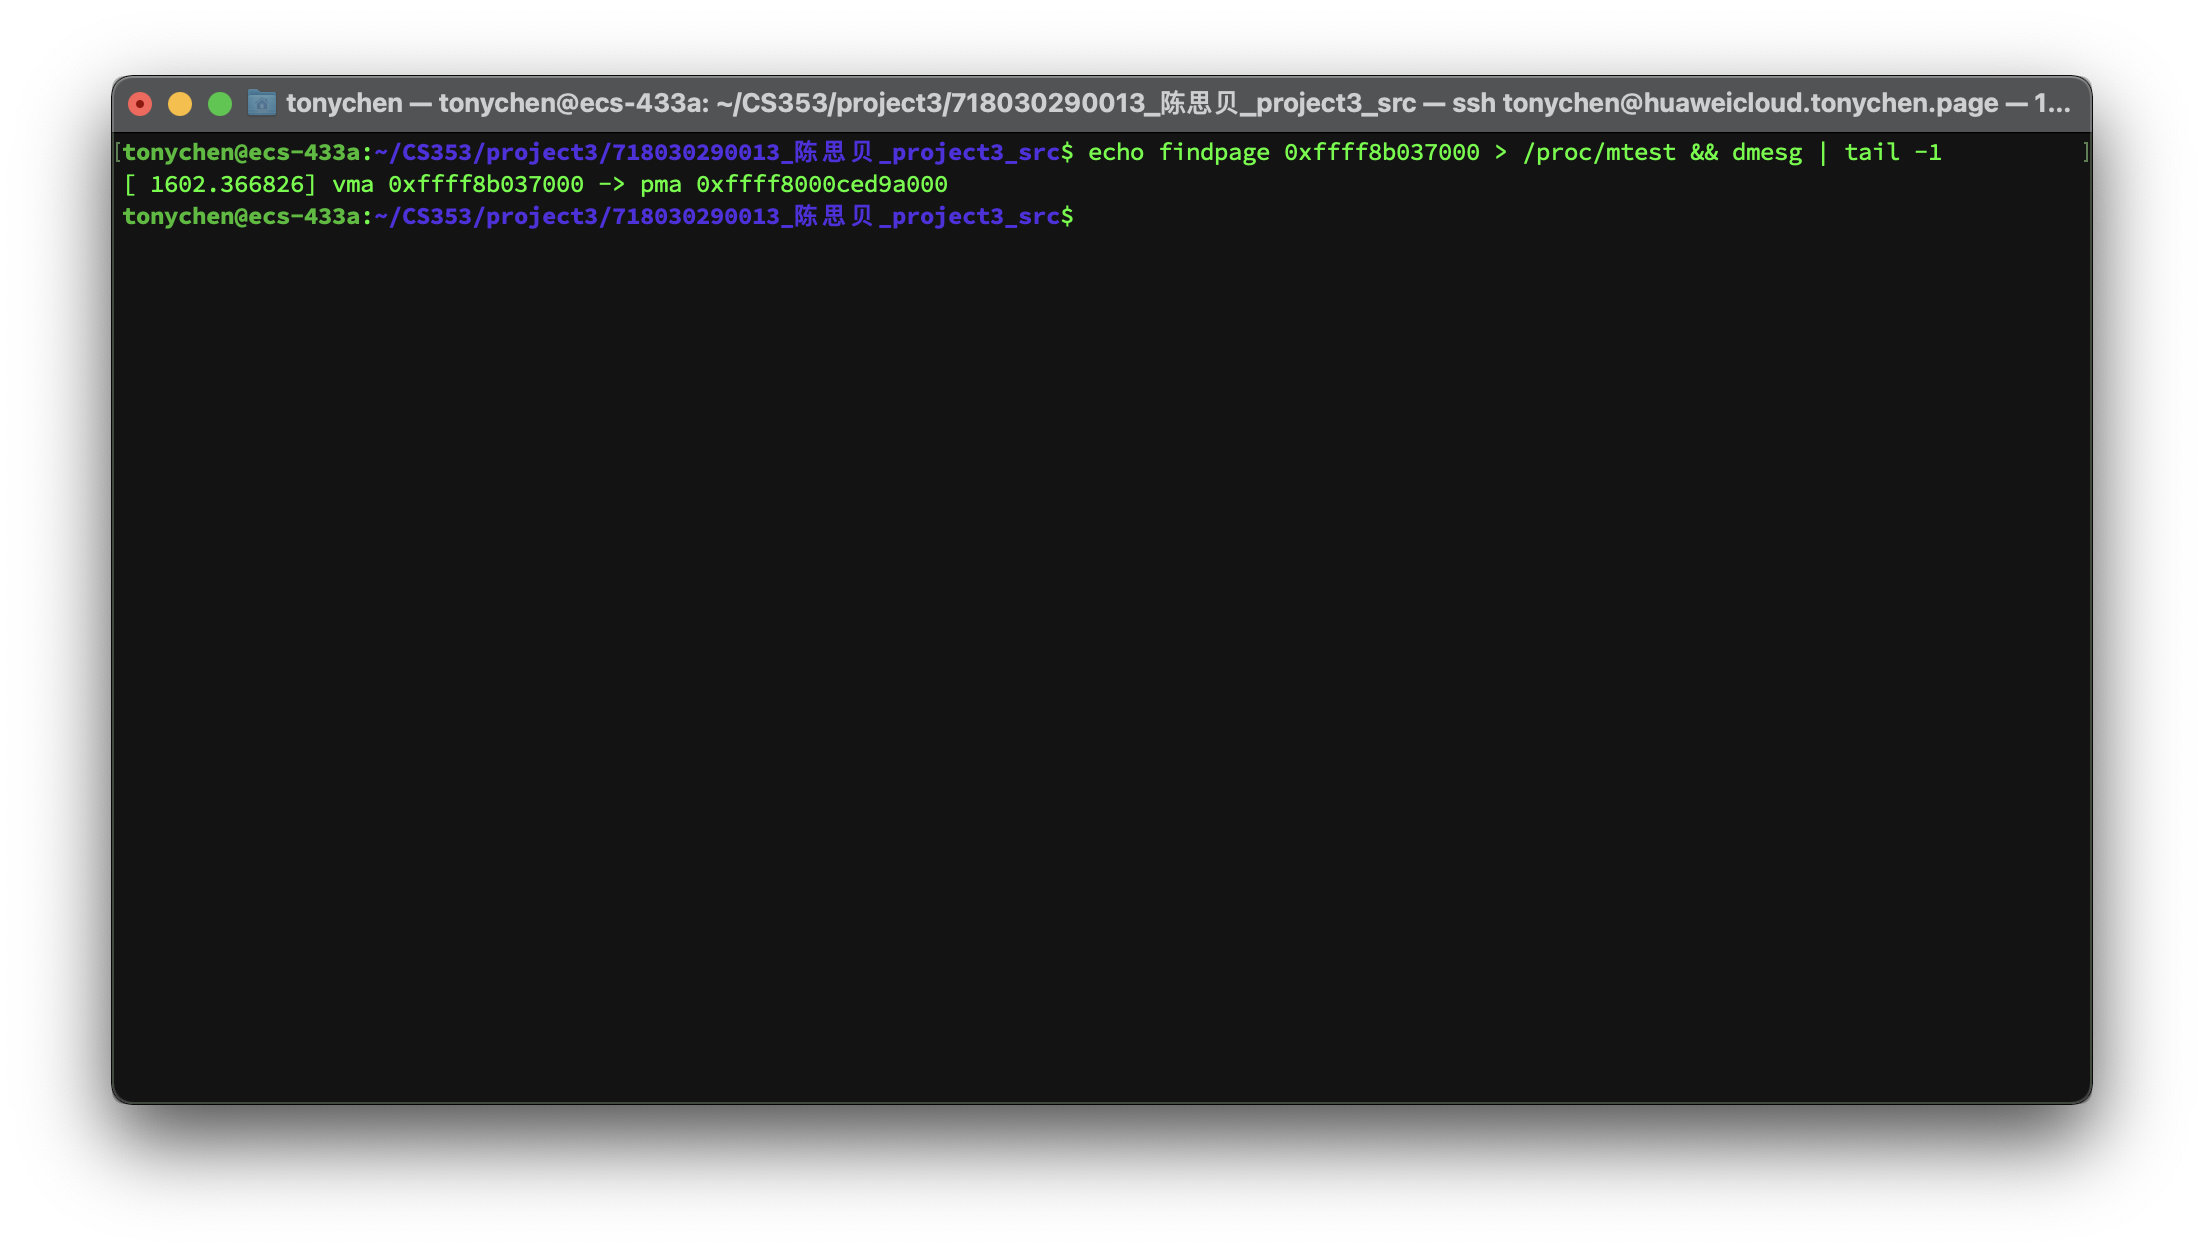
\includegraphics[width=15cm,keepaspectratio]{images/findpage.png}
        \caption{\texttt{findpage}运行结果}
        \label{fig:findpage}
    \end{figure}

    \begin{figure}[h!]
        \centering
        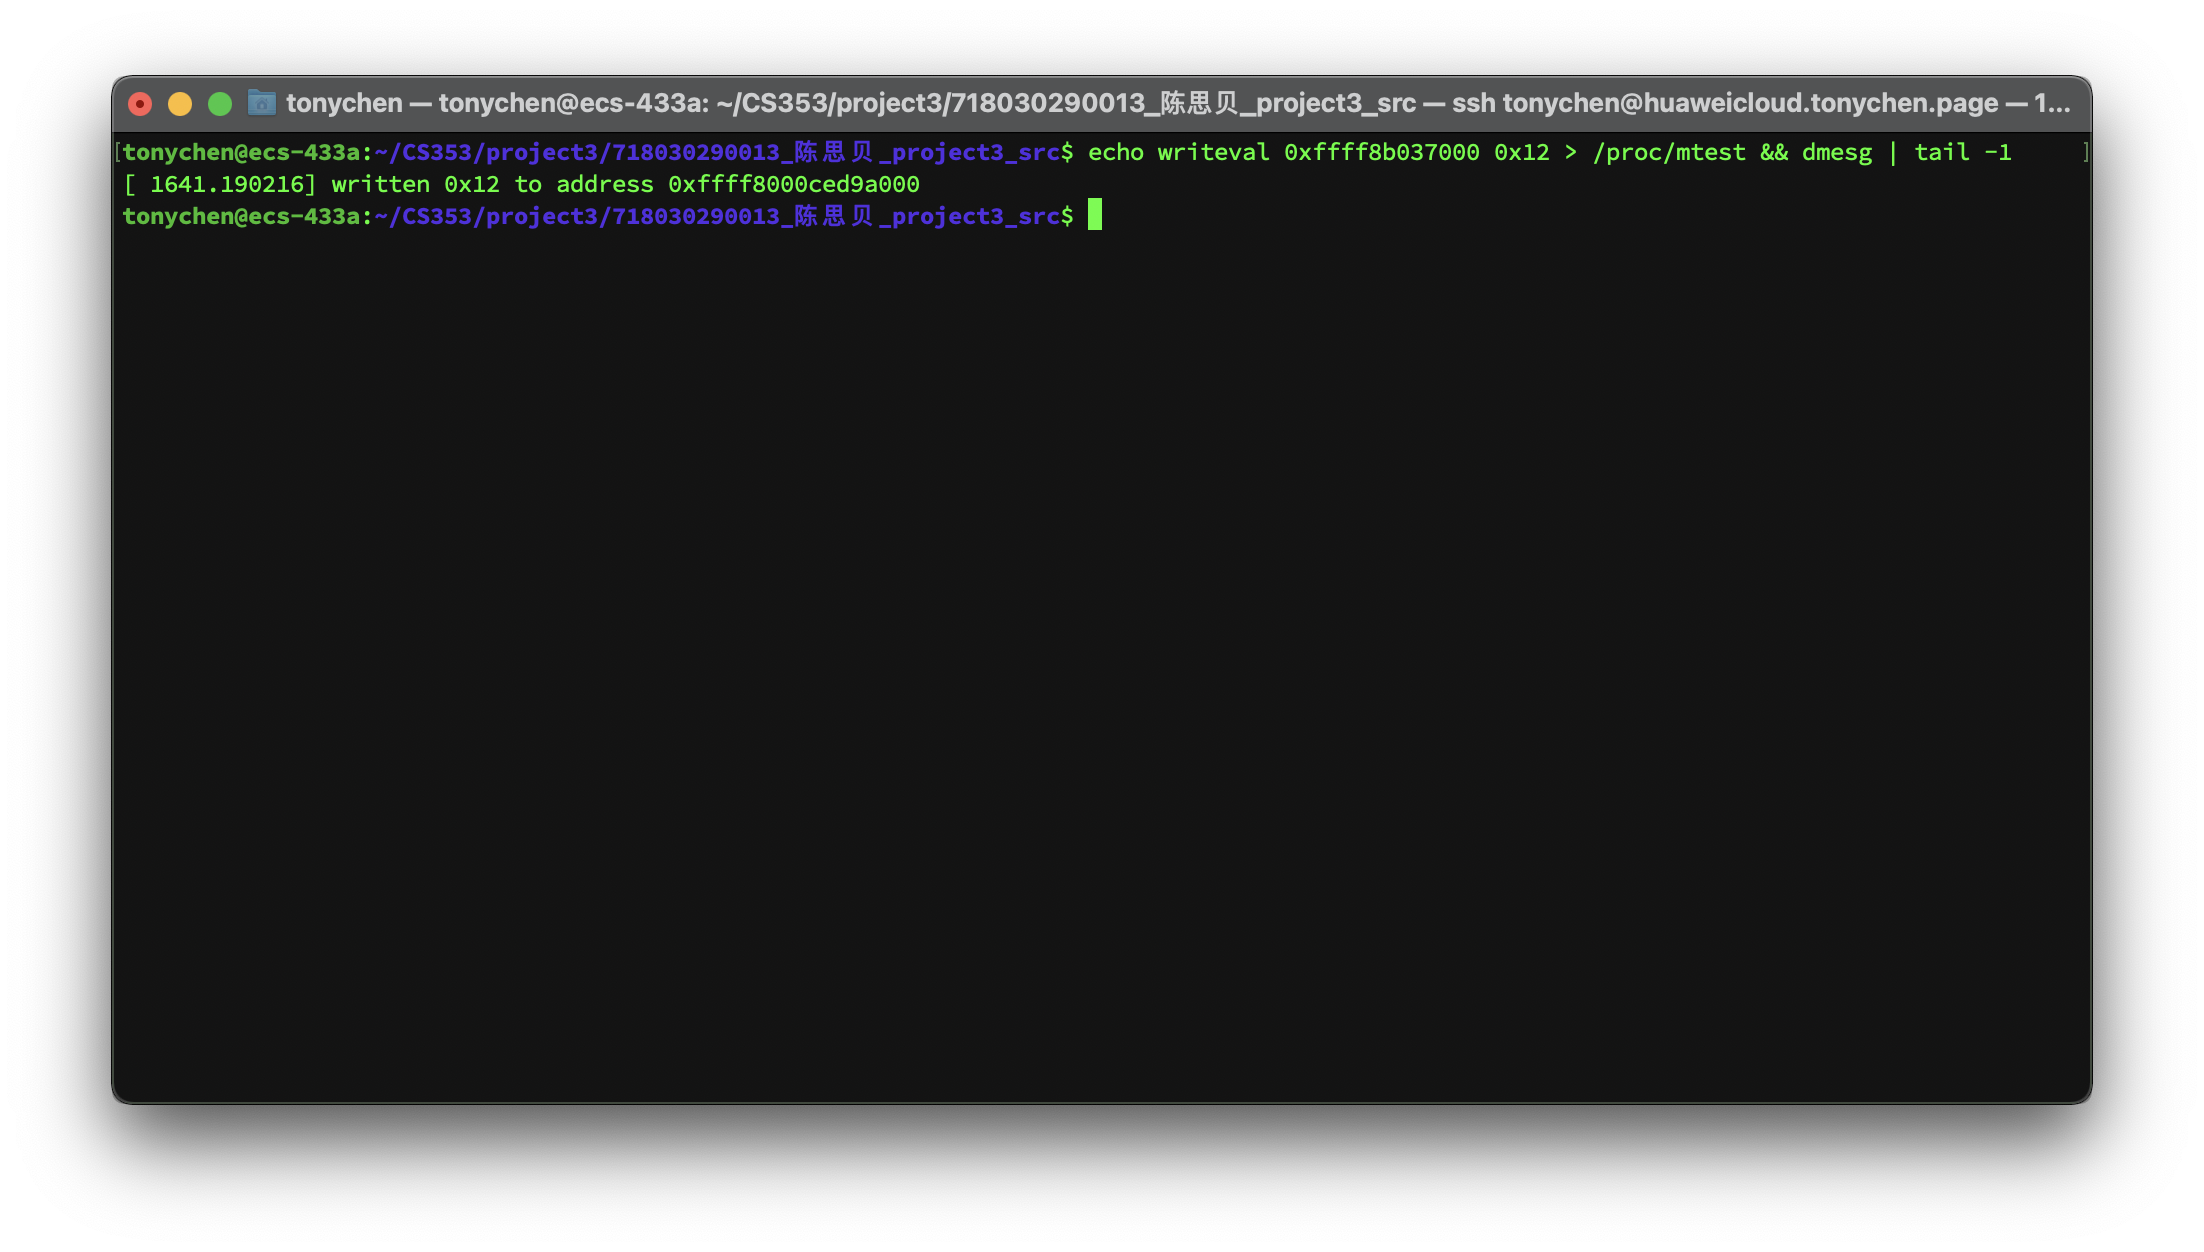
\includegraphics[width=15cm,keepaspectratio]{images/writeval.png}
        \caption{\texttt{writeval}运行结果}
        \label{fig:writeval}
    \end{figure}

    \section{实验心得}
    本次实验基于Linux内核的内存管理机制。通过对四层内存分页的逐级追踪解出虚拟内存与物理内存地址的对应关系。同时可以根据vma的不同变量的值,判断出模块对该块内存的权限状态。通过对内存物理地址的直接操作,可以做到对变量的直接输出与写入。通过本次实验,对Linux的内存管理方式有了更深刻的了解。在更新的内核中,Linux采用了更先进的五层内存分页,增加了支持的最大内存容量,但其计算原理与四层内存分页也是大同小异的。

\end{document}